\documentclass[11pt]{article}

\usepackage{amsmath,amssymb,amsfonts}
\usepackage{dsfont}
\usepackage{listings}
\usepackage{xcolor}
\usepackage{svg}
\usepackage{graphicx}
\usepackage{bbm}
\usepackage{float}
%\usepackage{hyperref}
\usepackage{subfig}
\usepackage[breaklinks=true,colorlinks,citecolor=black,linkcolor=gfGG,urlcolor=gfFP]{hyperref}
% http://www.colourlovers.com/palette/92095/Giant_Goldfish
\definecolor{gfCD}{HTML}{69D2E7} % Cloudless Day
\definecolor{gfSP}{HTML}{A7DBD8} % Sunken Pool
\definecolor{gfBS}{HTML}{E0E4CC} % Beach Storm
\definecolor{gfGG}{HTML}{F38630} % Giant Goldfish
\definecolor{gfFP}{HTML}{FA6900} % Food Pills

\definecolor{codegreen}{rgb}{0,0.6,0}
\definecolor{codegray}{rgb}{0.5,0.5,0.5}
\definecolor{codepurple}{rgb}{0.58,0,0.82}
\definecolor{backcolour}{rgb}{0.95,0.95,0.92}
\lstdefinestyle{mystyle}{
    backgroundcolor=\color{backcolour},
    commentstyle=\color{codegreen},
    keywordstyle=\color{magenta},
    numberstyle=\tiny\color{codegray},
    stringstyle=\color{codepurple},
    basicstyle=\ttfamily\footnotesize,
    breakatwhitespace=false,
    breaklines=true,
    captionpos=b,
    keepspaces=true,
    numbers=left,
    numbersep=5pt,
    showspaces=false,
    showstringspaces=false,
    showtabs=false,
    tabsize=2
}

\setlength{\topmargin}{-.5in} \setlength{\textheight}{9.25in}
\setlength{\oddsidemargin}{0in} \setlength{\textwidth}{6.8in}

%\newcommand*{\SOLVE}{}%

\renewcommand{\vec}[1]{\mbox{\boldmath$#1$}}
\newcommand{\mm}[1]{\mathbf{#1}}

\newcounter{ProblemNum}
\newcounter{SubProblemNum}[ProblemNum]

\renewcommand{\theProblemNum}{\arabic{ProblemNum}}
\renewcommand{\theSubProblemNum}{\alph{SubProblemNum}}

\newcommand*{\anyproblem}[1]{\section*{#1}}
\newcommand*{\problem}[1]{\stepcounter{ProblemNum} %
   \anyproblem{Problem \theProblemNum \; (#1 points)}}
\newcommand*{\soln}[1]{\subsection*{#1}}
\newcommand*{\solution}{\soln{Solution}}
\newenvironment{solutions}
  {\section[Solution]{\textcolor{red}{Solution}}\color{red}}
  {\normalcolor}
\renewcommand*{\part}{\stepcounter{SubProblemNum} %
  \soln{Part (\theSubProblemNum)}}
\renewcommand{\theenumi}{(\alph{enumi})}
\renewcommand{\labelenumi}{\theenumi}
\renewcommand{\theenumii}{\roman{enumii}}
\let\endsection\relax
\let\endsubsection\relax

\graphicspath{
{.}
}
\lstset{style=mystyle}

\begin{document}

\Large
\noindent{\bf CS4851/6851 IDL\:Homework 6 \hfill \today}
\medskip\hrule

\vspace{20pt}

Note: All coding problems to be submited with Github Link. Do not Upload the files/folder. Use git commands only.

Note: this is the distribution of questions:
\begin{enumerate}
  \item Question 1 to Question 3: Required for everyone.
  \item Question 4 to Question 5:  Bonus question for both Graduate Students and Undergraduate Students
\end{enumerate}


\problem{10}
We can represent the words in a vocabulary with binary vectors that have dimension of the number of words in the vocabulary and all values set to zero except the one value that corresponds to the index of the given word in the sorted version of this vocabulary. This is the so called one-in-K or one-hot encoding.

\begin{enumerate}
  \item Describe a representation of a document with a vector. (Think of a representation that is based on the one-hot encoding of the words in that document and has the same dimension as a single word (size of the vocabulary).)
  \item Explain why this representation is problematic:
    \begin{enumerate}
    \item  Simple sentence or two 
    \item  Examples of the problem(s)
    \end{enumerate}
  \item Provide atleast two more options to fix this problem.
\end{enumerate}
\problem{30}
A recurrent network in Figure~\ref{fig:RNN} takes a sequence of integers as an input and at the end of the sequence, on the last element produces a number between 0 and 1. What does a 0 mean? What does a 1 mean?  Describe which function this network is computing (what is the meaning of this function). Assume all biases are 0, and make sure the hidden state is initialized to 0 as well. Note, the inputs, the weights, and the hidden state are just scalars in this RNN.
\svgsetup{inkscapelatex=false}
\begin{figure}[!h]
  \centering
      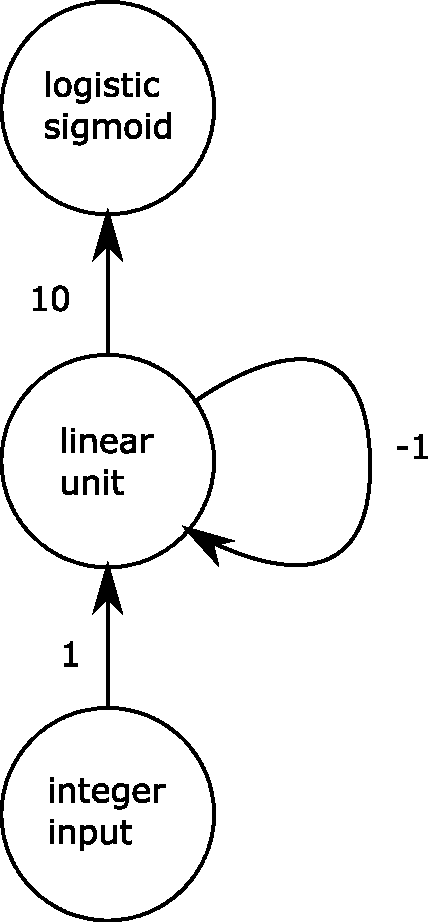
\includegraphics[width=0.2\linewidth]{RNN}
      \caption{The RNN for Problem~2 }
      \label{fig:RNN}
\end{figure}

\problem{20}
We have learned about regularization in image processing. How does regularization help in the context of Recurrent Neural Networks?

\vspace{10mm}
\noindent\rule[0.5ex]{0.45\linewidth}{1pt} Bonus for both  undergraduates and graduates beyond this line.


\problem{40} How is teacher forcing ratio more accurate than the model output for a sequence of inputs? How can we use teacher process to parallelize the computation?


\problem{40} Write a report on one of the following topics: 

\begin{enumerate}
  \item  Attention Is All You Need
  \{https://arxiv.org/pdf/1706.03762.pdf\}
  \item Transformers: \{https://arxiv.org/pdf/1910.03771v5.pdf\}
\end{enumerate}

% \vspace{2px}
\end{document}

%%% Local Variables:
%%% mode: latex
%%% TeX-master: t
%%% End:  
